%!TEX root = ../../../template.tex

\section{Air Pollution Monitoring Techniques}%
\label{sec:intro_air_pollution_monitoring_techniques}

There is no doubt that \gls{AP} is a global threat that affects
everyone, both in personal terms (through the degradation of their
health) and in societal terms, through the investments and limitations
that we as a whole have to commit to in order to prevent larger,
unmanageable problems. Reducing \gls{AP} is a priority and a requirement
for today's modern societies. This demands immediate and effective
actions, which in turn imply that we have a solid and profound
understanding of how pollutants are created, transported and transformed
in the atmosphere. The scale on which these interventions must be
conducted requires them to be made on a concerted and collaborative
manner, and always leveraged by technological
development~\cite{EEA2019}. Many of the air pollutants cannot be
detected solely by our senses, or even if they can is at already
dangerous concentrations. Technology is therefore a prerequisite to our
fighting the problem of \glsxtrlong{AP}~\cite{Vallero2014}.

Pollution monitoring is itself based on the ability of a given
measurement method to determine concentrations for trace gases, aerosols
or radiation quantities. As with many other test techniques, in various
fields, pollution monitoring techniques have three very important
aspects to verify. The first of which is sensitivity, and also the most
demanding. Important trace gases in atmospheric chemistry have sometimes
vestigial concentrations, and the ability to correctly detect them is
many times a technical challenge. The second most important is
specificity, which is the ability of an atmospheric measurement to
measure each compound independently, without a component influencing
another component's measurement either positively or negatively.
Finally, any usable monitoring technique must be sufficiently precise as
to provide valid measurements.

\glsxtrlong{AP} monitoring techniques and devices are too many to address
them all in this document. However, a small introduction to the topic is
in order. A valid point of entry in this discussion would be a broad
categorisation of monitoring techniques with regard to the proximity
with which they are designed to interact with the target pollutant.
As with the case of fire detecting systems, reported
in~\cite{ValentedeAlmeida2017}, atmospheric pollution monitoring systems
can be divided into three broad categories, which are further divided as
in~\ref{fig:pollution_monitoring_tree}:

\begin{description}
    \item[In-situ systems] localised sensors that are influenced by
        gases in their immediate vicinity;
    \item[Large area (open path) systems] able to evaluate the
        atmosphere around them (normally through somekind of optical
        measurement) up to a few km;
    \item[Remote systems] placed in satellites, which were designed to
        perform a more global analysis of the atmosphere and identify
        larger-scale trends;
\end{description}

\begin{figure}[htpb]
    \centering
    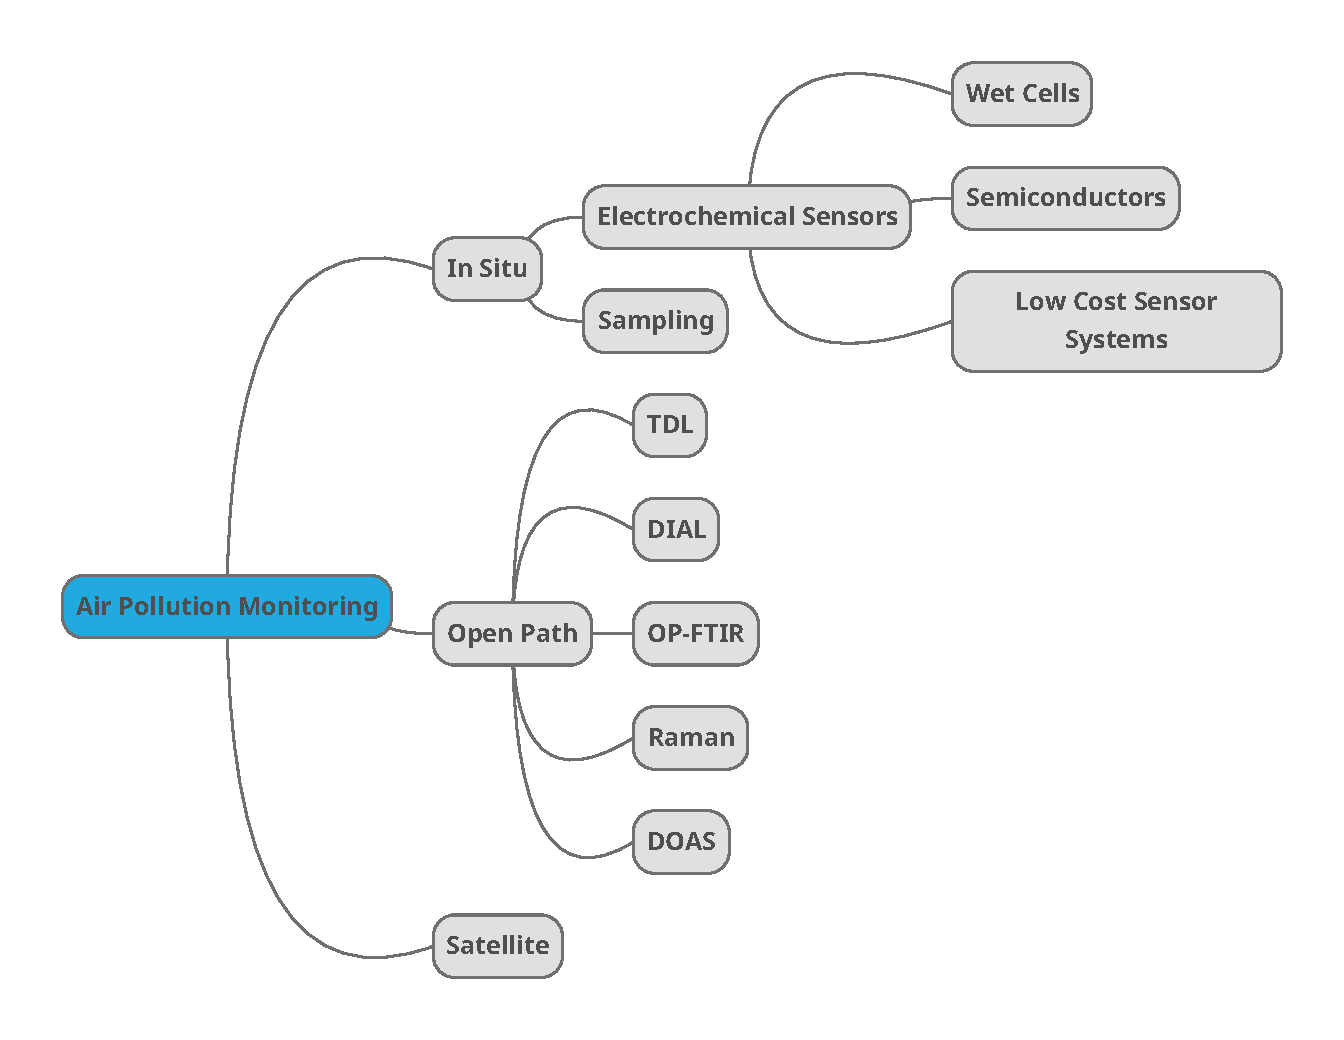
\includegraphics[width=.8\textwidth]{img/pdf/air_pollution_monitoring_tree.pdf}
    \caption{A tree diagram providing a general overview of the various
    types of atmospheric pollution monitoring systems. }%
    \label{fig:pollution_monitoring_tree}
\end{figure}

Sampling studies are still regarded as the gold standard for atmospheric
pollution monitoring. They are fundamentally different from the other
methods, because there is an important time gap between collection and
analysis. Sampling methods cannot provide real time information on
atmospheric composition. The gaseous analyte is moved into a collection
medium before being transported to the laboratory, where a very powerful
analytical method such as mass spectroscopy or chromatography is used to
retrieve the chemical composition of the sample. The use of this kind of
technique determines the importance of sampling methods in the study of
the atmosphere's composition, but they also make them quite inconvenient
for day to day use~\cite{Vallero2014}.

A much more convenient solution comes in the shape of electrochemical
sensors. They were highly popularised in recent decades through their
usage in the field of industrial hygiene~\cite{Clark1997}. The first
generation of these sensors were called wet cells. The basic design for
an \gls{o2} sensor of this type is presented in
Figure~\ref{fig:electrochemical_wet_cell}. When an electromagnetic force
is applied to the cell, hydrogen appears at the cathode, and oxygen at
the anode. Conversely, when the cathode is subject to an oxygen
concentration and an appropriate electrolyte is used (for instance,
KOH), an electronic charged develops through the oxidation of the anode
into a hydroxide. If a load is presented to the system, the current
flowing through it is proportional to the partial pressure of oxygen in
the mixture~\cite{Dhall2021, Clark1997}~\todo{citation image - citicel}.

\begin{figure}[htpb]
    \centering
    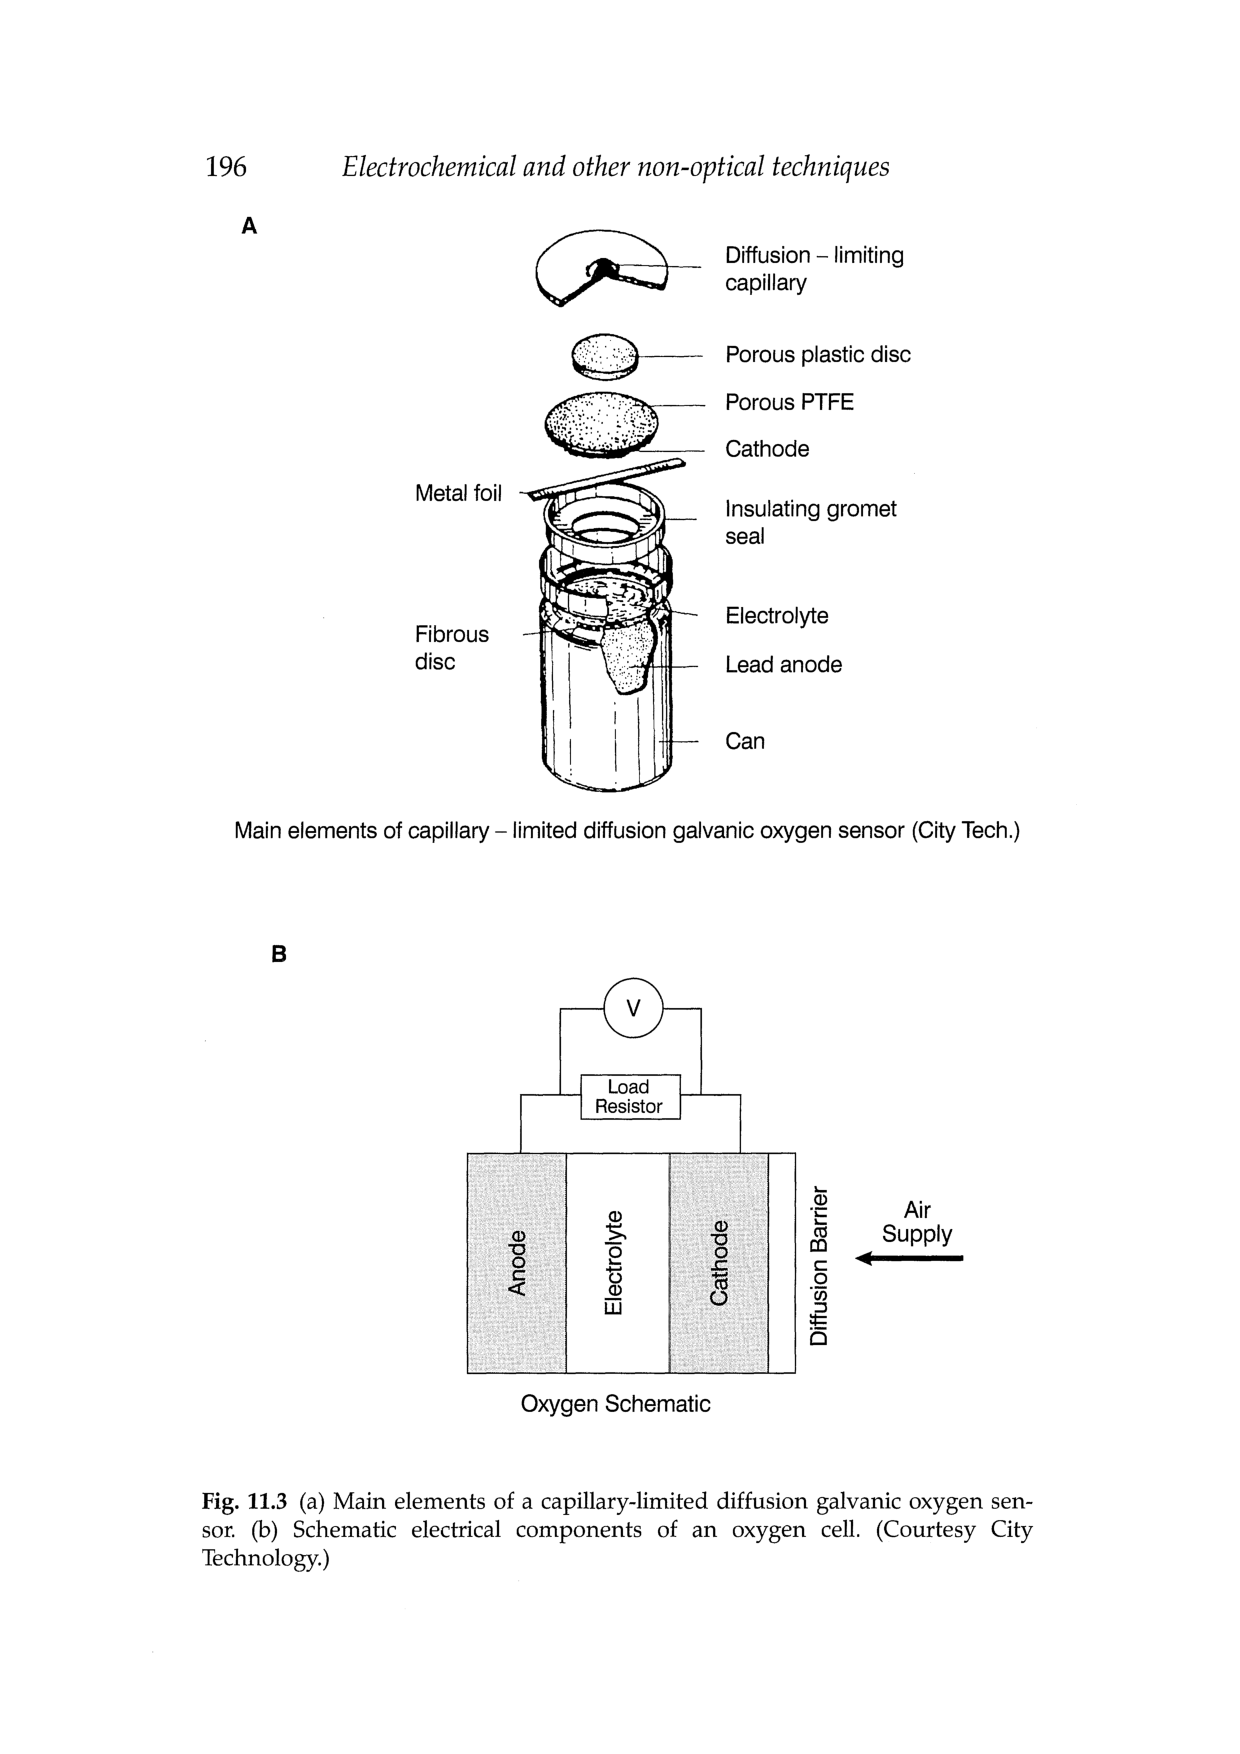
\includegraphics[trim=6cm 6.2cm 4cm 16cm, clip]{img/pdf/clark_193.pdf}
    \caption{An oxygen electrochemical sensor developed by Citi}%
    \label{fig:electrochemical_wet_cell}
\end{figure}

A similarly applicable technology is the use of semiconductor sensors.
These usually operate by the detection 



%\glsxtrlong{AP} monitoring techniques and devices are too many to address
%them all in this document. Besides, the physical principles involved are
%completely different from one to another, making it very difficult to
%make a broad generalization, other than the fact that they can be
%divided into local and remote sensing devices. The gold standard for air
%quality measurements remains those techniques in which a sample is
%collected in the field and then taken to the laboratory to be analyzed
%by very powerful analytical methods such as chromatography or mass
%spectroscopy. While undoubtedly providing the most accurate
%representation of the air composition at the time and place the sample
%was collected, it is also true that this method's results are too slow
%to use regularly in the field~\cite{Vallero2014, Clark1997, Bishop1996}.

%Another very important air quality monitoring method is the use of
%electrochemical sensors. The first variants (wet cells) of this kind of
%sensor became very popular in the field of industrial hygiene, where
%they were applied in many portable flue gas analyzers. They were very
%attractive to companies worldwide given their potential for very low
%costs in comparison to optical or other more complex techniques. Apart
%from the oxygen wet cell sensor, that has a slightly different
%configuration, these electrochemical devices are comprised of three
%electrodes - a sensing electrode, a counter electrode and a reference
%electrode - separated by a thin layer of electrolyte. The gas that is
%diffused to the surface of the electrode is either oxidized or reduced,
%thus changing the systems electrical properties, in a way that is then
%captured by an amplification circuit~\cite{Clark1997}.

%Wet cell electrochemical sensors were the precursors of the now more
%common solid state sensors. These sensors are the ones that we see in
%every subterranean parking lot, measuring several traffic related gases
%such as \gls{co}, \gls{co2} or \gls{no2}. In general semiconductor gas
%detectors are comprised of two modules: a receptor and a transducer (see
%Figure~\ref{fig:semiconductor_sensor}). The receptor has in its
%composition a material (or set of materials) that, in contact with the
%target gas, induces a change in the systems inherent properties (work
%function, dielectric constant, resistance, etc.) or emits heat or light.
%The transducer is a device or circuit that converts the receptor's
%changes into an electrical signal~\cite{Clark1997, Bishop1996,
%Vallero2014}.

%\begin{figure}[htpb]
%    \centering
%    %\includegraphics[trim=left bottom right top, clip]{file}
%    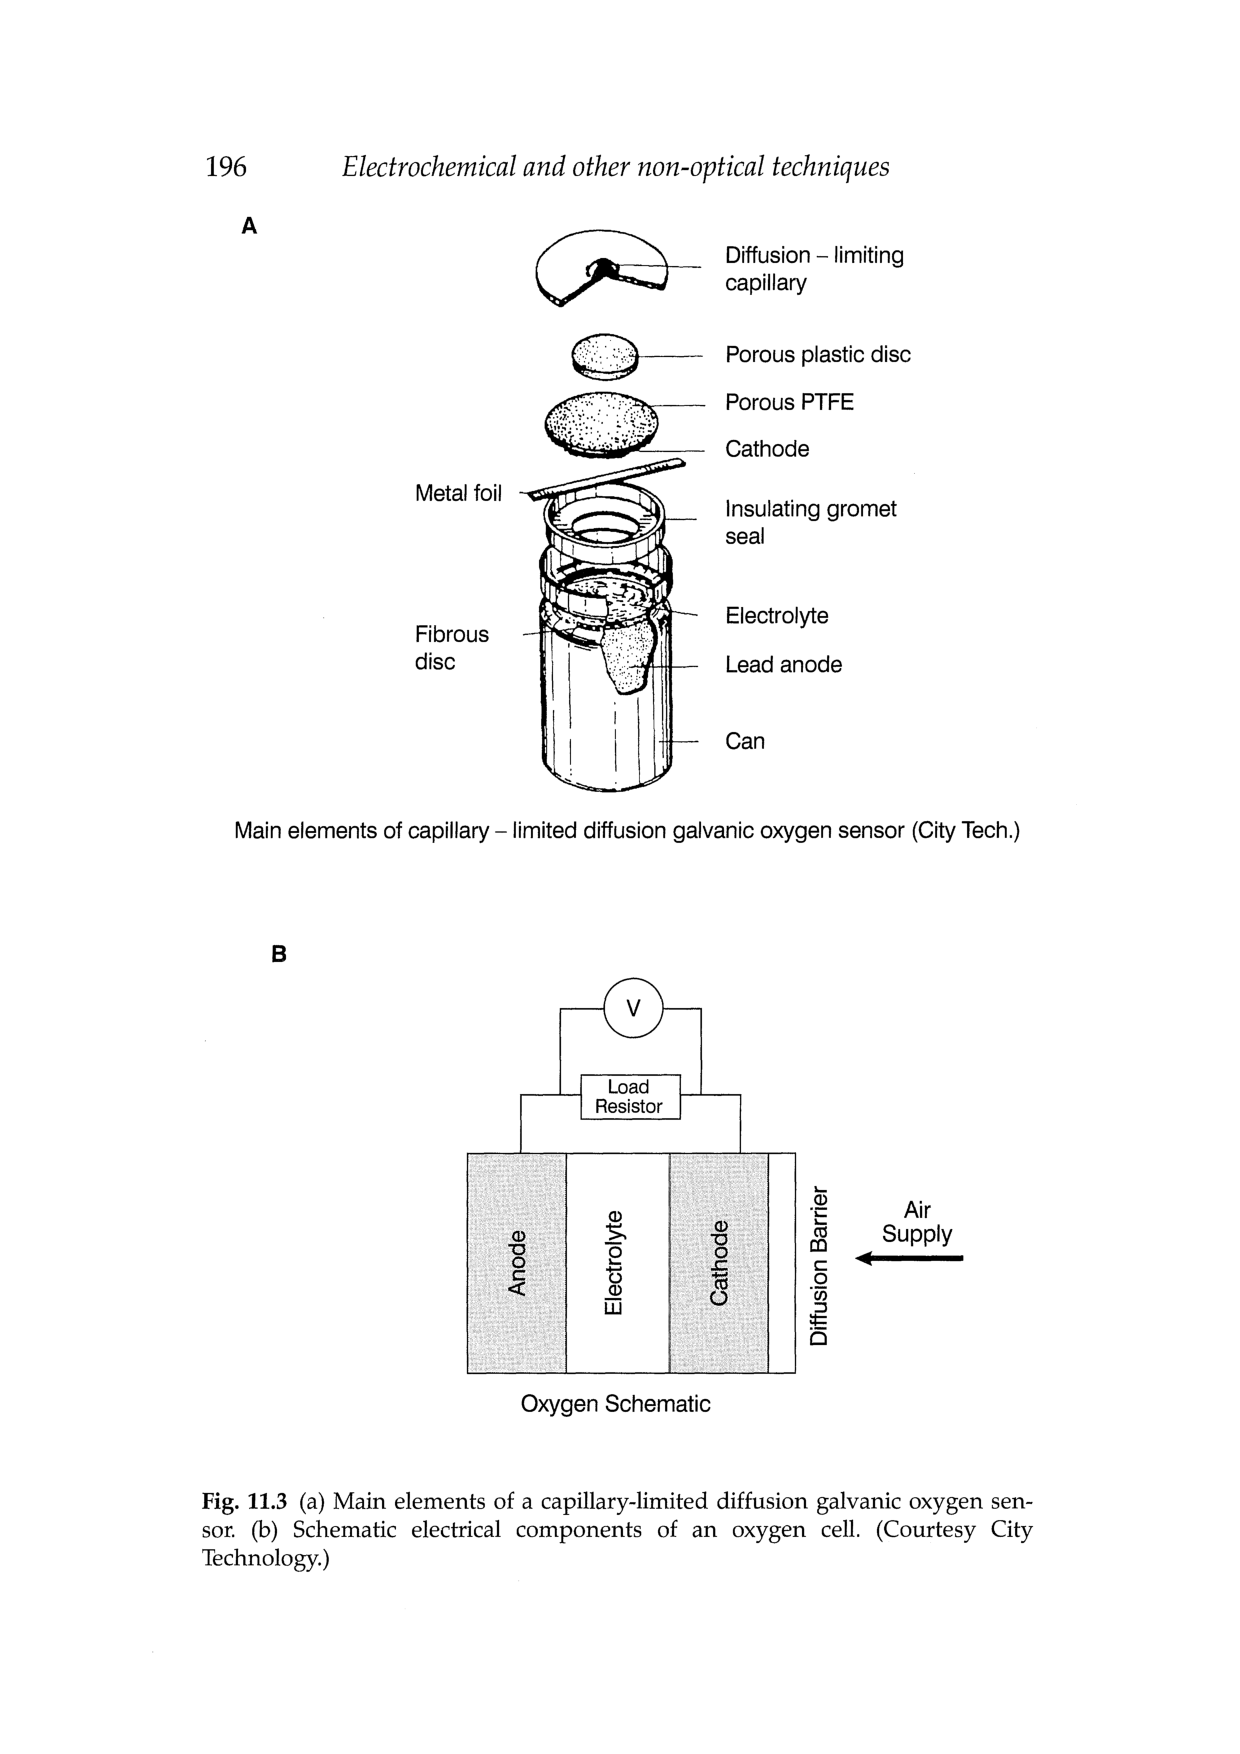
\includegraphics[trim=6cm 6.2cm 4cm 16cm, clip]{img/pdf/clark_193.pdf}
%    \caption{Semiconductor electrochemical sensor basic structure. There
%    are many examples of this type of sensors, but in general they
%    follow this architecture~\cite{Clark1997}.}
%    \label{fig:semiconductor_sensor}
%\end{figure}

%Optical (spectroscopic) systems are fundamentally different from the
%other techniques that have already been presented. They can be used to
%perform remote sensing measurements (as far as being used for
%measurements aboard satellites). In the last few decades, these
%techniques have gained a lot of ground in atmospheric research, due to
%their high sensitivity and specificity and the universality of their
%applicability. Spectroscopic methods are based on Lambert-Beer's law
%(see Section~\ref{sec:doas} for a more thorough explanation), and make
%use of the fact that the way in which gases interact with light is well
%known and follows an exponential expression. There are many
%spectroscopic techniques for measuring \gls{AP}. One of the most
%important atmospheric analysis methods, and especially in what concerns
%this document, is \gls{DOAS}. While it is based on the same mathematical
%formulation as the other spectroscopic methods, it is also based on
%other factors, which shall be discussed in Section~\ref{sec:doas}.

